\chapter{Perspectividades}
\label{C7}
A lo largo de este capítulo estudiaremos un tipo especial (y muy importante) de homografías, las llamadas \ti{perspectividades}. Para que el ánimo no decaiga, comencemos con un resultado bonito.
\section{Teorema de Desargues}
\label{C7_Desargues}
En esta sección enunciaremos y demostraremos un resultado clásico de la geometría proyectiva, el llamado ``Teorema de Desargues''. Este teorema es de gran interés por multitud de razones. Una de ellas es que es un teorema \ti{autodual} (como luego veremos).

Comencemos con una pequeña definición.
\begin{defi}[Triángulos en Perspectiva]
	Dados dos triángulos (a los que denotaremos por sus vértices) $ABC$, $A'B'C'$, se dice que están \ti{en perspectiva} si se verifica:
	\[AA'\cap BB'\cap CC'=O\]
\end{defi}
El teorema de Desargues nos da una condición necesaria y suficiente para que dos triángulos se encuentren en perspectiva.
\begin{theo}[Teorema de Desargues]
	\label{C7_teo_desargues1}
	Dados dos triángulos en el plano proyectivo $ABC$, $A'B'C'$ con vértices distintos. Consideremos los puntos:
	\[\begin{array}{c}
	Z=AB\cap A'B'\\
	Y=AC\cap A'C'\\
	X=CB\cap C'B'
	\end{array}\]
	Los tríangulos están en perspectiva si y solo si $X,Y,Z$ son colineales.
	\begin{figure}[h]
		\centering
		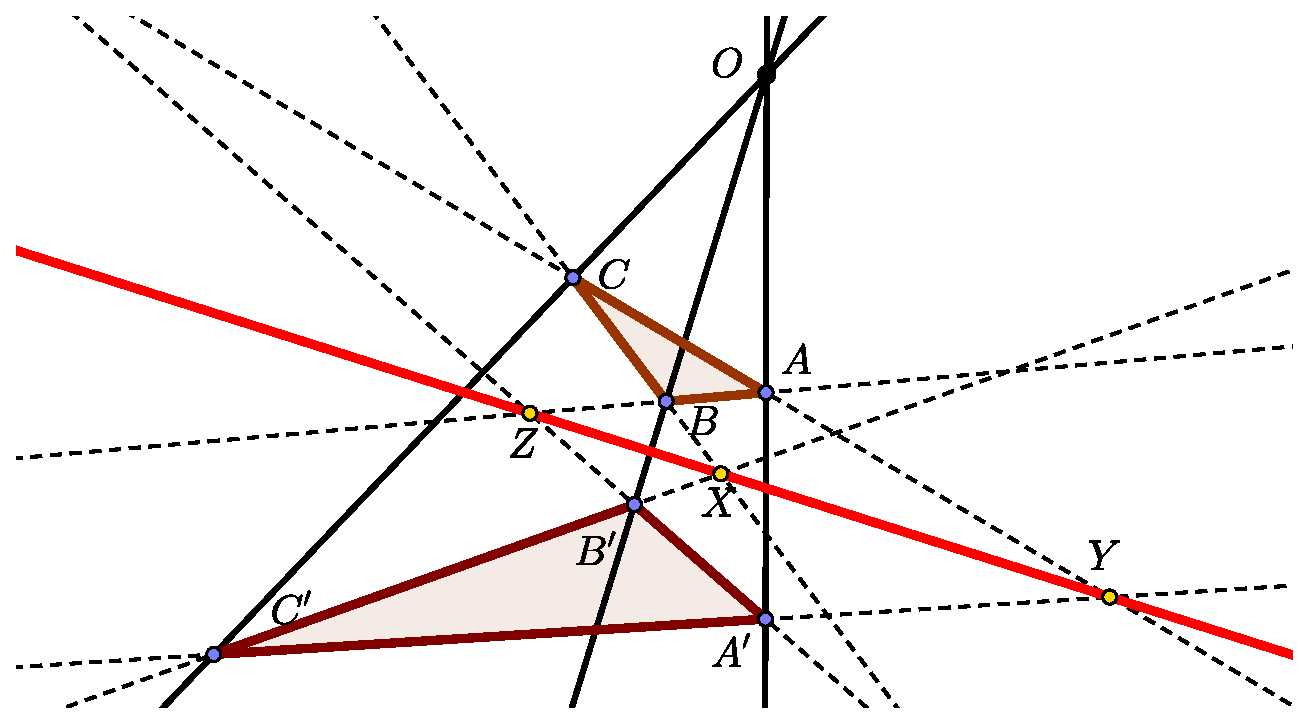
\includegraphics[scale=.45]{Graficos/desargues.eps}
		\caption{Ilustración del Teorema de Desargues.}
		\label{C7_img_desargues}
	\end{figure}
	
\end{theo}
\begin{proof}
	Suponiendo que los triángulos están en perspectiva, demostremos que los puntos $X,Y,Z$ son colineales. Para ello, demostraremos que sus representantes (independientemente de cuales escojamos) son linealmente dependientes.
	
	Antes de comenzar, fijemos notaciones:
	\[\begin{array}{ccc}
	& O=\class{\vec{o}} & \\
	A=\class{\vec{a}}   & B=\class{\vec{b}}   & C=\class{\vec{c}}\\
	A'=\class{\vec{a'}} & B'=\class{\vec{b'}} & C'=\class{\vec{c'}} 
	\end{array}\]
	
	Como los triángulos están en perspectiva, se tiene que los puntos $O,A,A'$ (distintos) están alineados, es decir, tienen representantes coplanarios, por ende, podremos escribir uno de estos representantes como combinación lineal de los otros. En este caso escribiremos:
	\[\vec{a'}=\lambda \vec{o}+\alpha\vec{a}\]
	Como los puntos son distintos, es claro que $\vec{a'}$ no se podrá escribir como múltiplo de un solo representante, esto significa que ambos coeficientes de la combinación lineal son no nulos, luego, dividiendo por $\lambda$ y renombrando (cometiendo cierto abuso de notación) al representante y a las variables obtenemos que:
	\[\vec{a'}=\vec{o}+\alpha\vec{a}\]
	Repitiendo esta misma jugada con los puntos $O,B,B'$ y $O,C,C'$ obtemos las identidades:
	\[\begin{array}{lr}
	\vec{b'}=\vec{o}+\beta\vec{b} \qquad&\qquad
	\vec{c'}=\vec{o}+\gamma\vec{c}
	\end{array}\]
	Una forma fácil de hallar un representante del punto $Z$ es restar los vectores $\vec{a'}$ y $\vec{b'}$. En efecto:
	\[\vec{a'}-\vec{b'}=\alpha\vec{a}-\beta\vec{b}=:\vec{z}\in\lengen{\vec{a'},\vec{b'}}\cap\lengen{\vec{a},\vec{b}}\stackrel{\eqref{C1_eq_explicitaEngendrados}}{\ra}\class{\vec{z}}\in A'B'\cap AB=:Z\]
	De nuevo, repetimos esta idea para hallar representantes de los puntos $X$ e $Y$, obteniendo:
	\[\begin{array}{lr}
	\vec{y}:=\vec{c'}-\vec{a'}=\gamma\vec{c}-\alpha\vec{a}\qquad&
	\qquad \vec{x}:=\vec{b'}-\vec{c'}=\beta\vec{b}-\gamma\vec{c}
	\end{array}\]
	Veamos que los representantes escogidos de los puntos $X,Y,Z$ son linealmente dependientes, para ello basta con sumarlos. En efecto (compruébese):
	\[\vec{x}+\vec{y}+\vec{z}=0\]
	Lo que concluye la demostración de la primera implicación del teorema.
	
	Recíprocamente, los dioses nos reservan un pequeño presente, que hará valer, aún más si cabe, nuestros conocimientos acerca de dualidad. Resulta que, como ya adelantamos, el teorema de Desargues es un teorema \ti{autodual}. Esto quiere decir que, como ya sabemos, podemos optar por, en lugar de demostrar la otra implicación ``a pelo'', demostrar su dual. Sin embargo, resulta que al dualizar el enunciado de esta segunda implicación, obtenemos el enunciado de la primera (ya demostrada), por lo cual, acabamos de reducir un problema de complejidad desconocida, a una simple trivialidad. Es por esto que se suele decir que el recíproco del teorema de desargues es obvio por dualidad.
	
	La comprobación de que esto es así es un sencillo ejercicio para el cual se recomienda refrescar la sección \ref{C2_principioDualidadProyectiva}.
\end{proof}
Nótese que en la demostración de la primera implicación del teorema no se ha usado para nada la hipótesis de que los puntos se encuentren en el plano proyectivo, esto nos hace ver que dicho fragmento del teorema es válido para dimensión arbitraria (finita). Sin embargo, recordemos que a la hora de comprobar que, efectivamente, el dual del enunciado de la segunda implicación era el enunciado de la primera, esta hipótesis nos fue crucial.

Aunque la demostración que hemos visto del teorema de Desargues no es especialmente enrevesada ni difícil, quizá si peque de no ser muy intuitiva y de tener cierta componente de idea feliz, es por esto que veremos otras dos demostraciones del mismo teorema al final del capítulo.
\section{Perspectividades}
\label{C7_Perspectividades}
Comencemos ya con la parte central del capítulo, el estudio de las \ti{perspectividades}. Comencemos por la definición.
\begin{defi}[Perspectividad]
	\label{C7_defi_perspectividad}
	Una homografía $h:l\to l'$, donde $l$ y $l'$ son rectas distintas de $\proy^2$ se dice \ti{perspectividad} si es la restricción a $l$ de la proyección cónica de centro $O(\not\in l\cup l')$ en $l'$. es decir:
	\[\left.\begin{array}{ccc}\proy^2\setminus{O}&\stackrel{\pi_O}{\to}&l'\\p& \mapsto & Op\cap l'\end{array}\right\}\leadsto h\equiv \pi_O|l\]
\end{defi}
Obsérvese que con la definición \ref{C7_defi_perspectividad} no hemos hecho más que revisitar el viejo ejemplo \ref{C4_exa_fabricaHomografias}.
\begin{figure}[h]
	\centering
	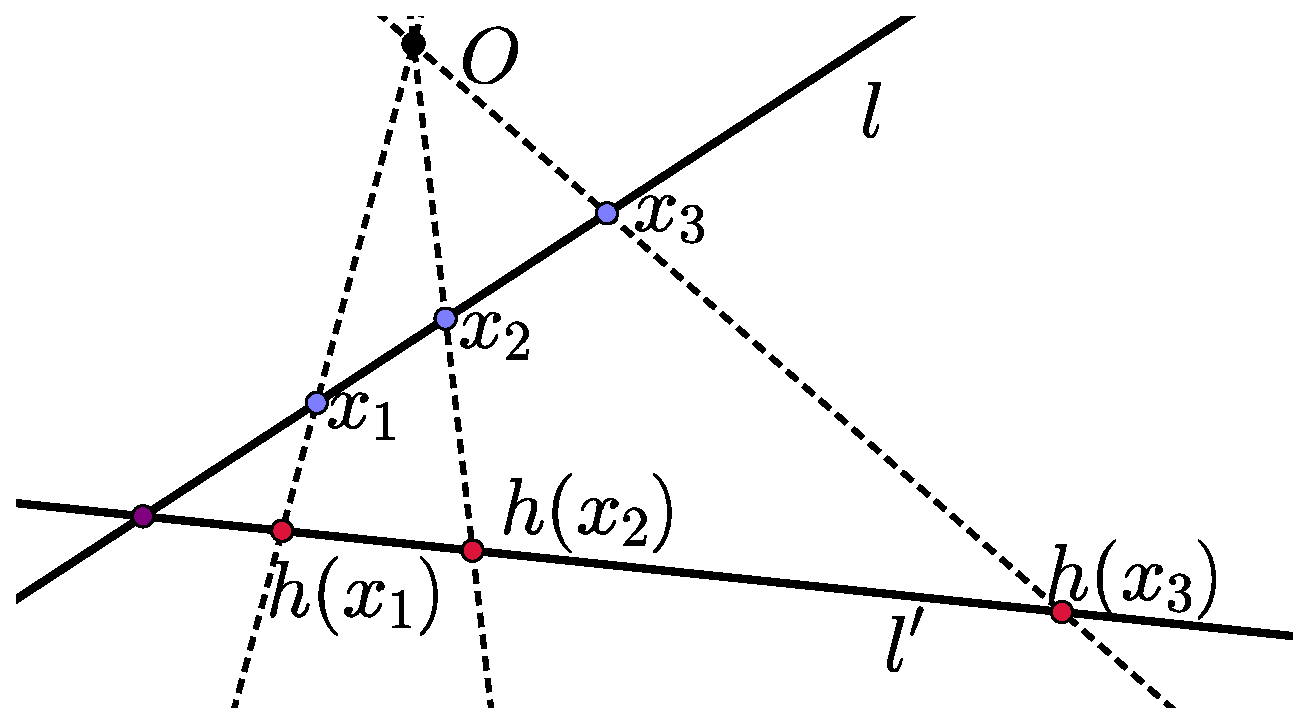
\includegraphics[scale=.3]{Graficos/perspectividad.eps}
	\caption{Ilustración de una Perspectividad.}
	\label{C7_img_perspectividad}
\end{figure}

La comprobación de ser perspectividad parece bastante engorrosa, por ello, los geómetras del mundo se pusieron a trabajar y obtuvieron la siguiente caracterización, que si uno mira la figura \ref{C7_img_perspectividad}, es bastante intuitiva.
\begin{prop}[Caracterización de las Perspectividades]
	\label{C7_prop_caracterizacionPerspectividades}
	Una homografía $h:l\to l'$ es perspectividad si y solo si deja fijo el punto $c:=l\cap l'$.
\end{prop}
\begin{proof}
	Supongamos que la homografía deja fijo el punto $c$. Tomemos dos puntos distintos $P,Q$ de la recta $l$ distintos de $c$. Consideremos asimismo sus imágenes $P'=h(P)$ y $Q'=h(Q)$. Es evidente (por estar en $\proy^2$) que las rectas $PP'$ y $QQ'$ se cortarán en cierto punto $O$. Entonces, resulta que nuestra homografía $h$ coincide con la perspectividad de centro $O$ que va de $l$ a $l'$ en tres puntos distintos; $c, P, Q$. Como vimos en la proposición \ref{C5_prop_homografia3puntos}, que dos homografías de la recta coincidan en tres puntos, implica que estas son iguales, por ende, nuestra homografía $h$ es una perspectividad. El recíproco es obvio.
\end{proof}
La proposición \ref{C7_prop_caracterizacionPerspectividades} nos da una forma bastante cómoda de comprobar que una homografía es una perspectividad.
\subsection{Perspectividades y Dualidad}
Para terminar la sección, tratemos de dar una interpretación dual al concepto de perspectividad.

Como sabemos, los puntos de una recta del plano proyectivo se corresponden, por dualidad canónica, con un haz de rectas con cierta base.

Así pues, la interpretación dual de una homografía $h$ entre dos rectas $l$ y $l'$ será una aplicación $h^*$ entre dos haces de rectas $\text{Haz}(A)$ y $\text{Haz}(B)$.

Dicha aplicación enviará cada recta $x^*\in\text{Haz}(A)$ a otra recta $y^*\in\text{Haz}(B)$. Donde la recta $x^*$ se corresponde con el punto $x\in l$, y la recta $y^*$ es el dualizado del punto $y=h(x)\in l'$.

Pasemos ahora a dualizar la definición de perspectividad.
\begin{defi}[Perspectividad Dual]
	Una homografía $h^*$ entre dos haces de rectas se dirá \ti{perspectividad} si a cada recta $p^*$ del haz de partida le asigna $\engen{O^*\cap p^*,l'^*}$ donde $O^*$ es una recta que no pertenece a ninguno de los haces.
\end{defi}
\begin{figure}[h]
	\centering
	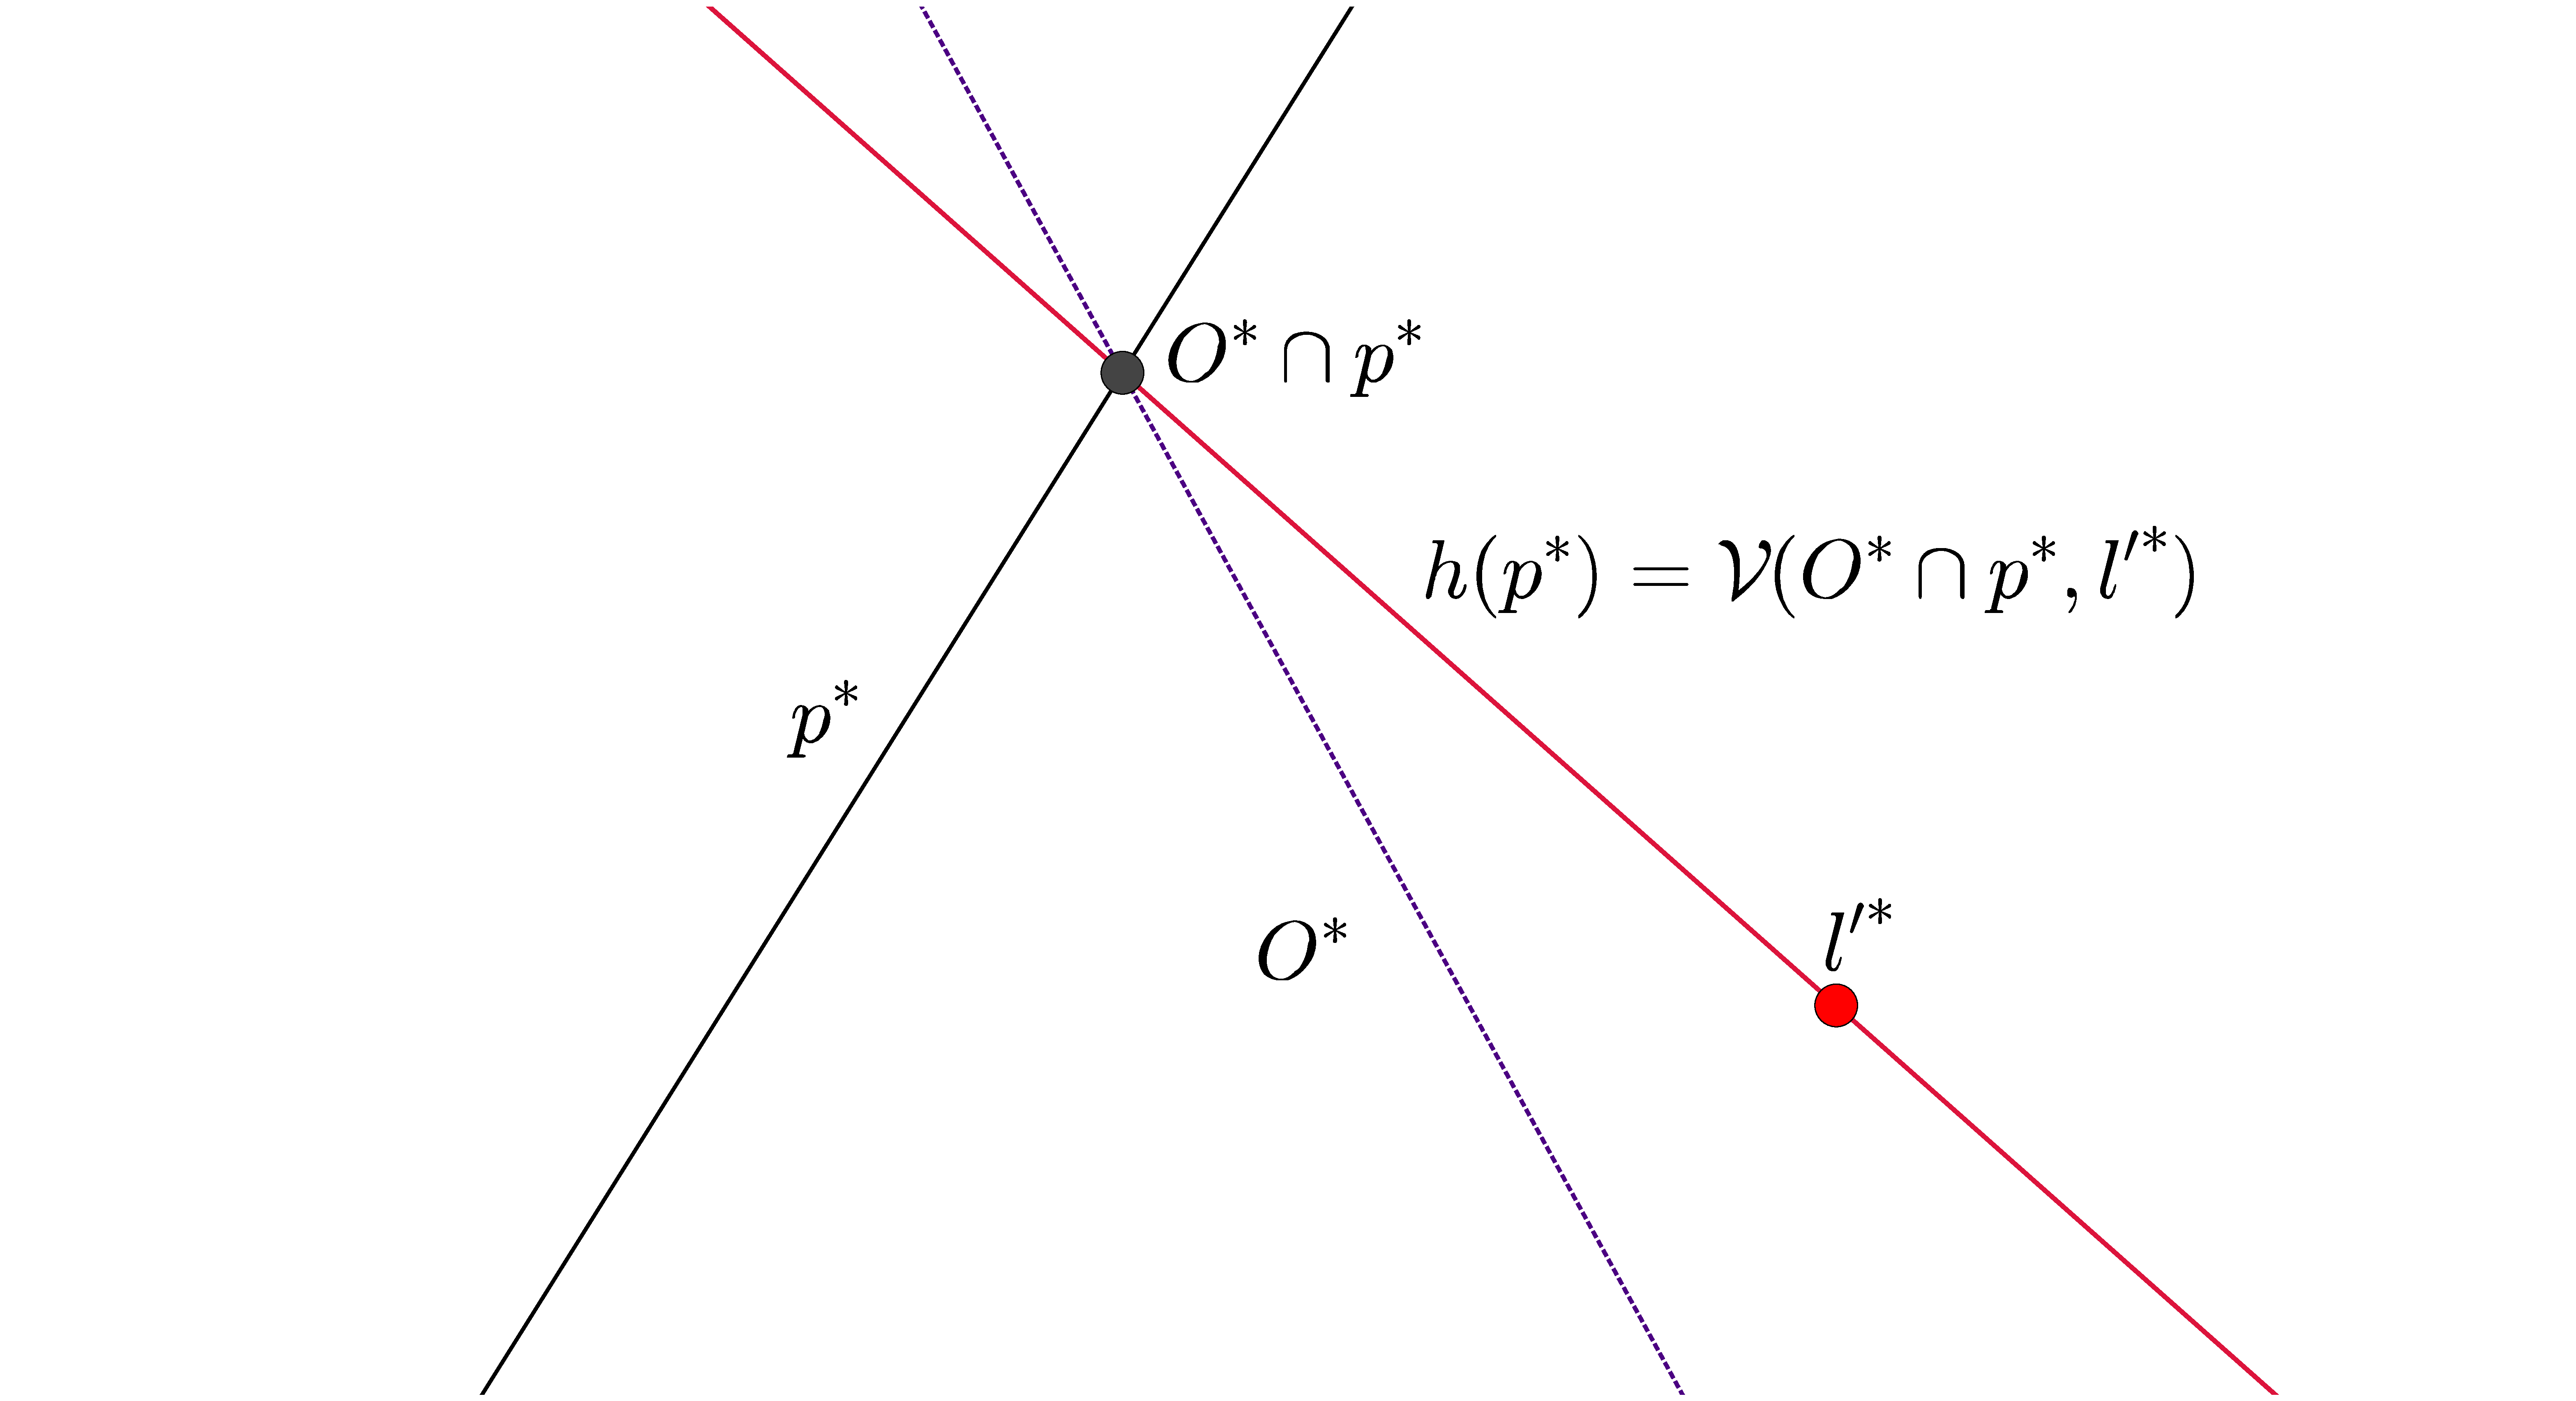
\includegraphics[scale=.1]{Graficos/perspectividadDual.eps}
	\caption{Ilustración de una Perspectividad Dual.}
	\label{C7_img_perspectividadDual}
\end{figure}
Hecho esto, podemos dualizar la proposición \ref{C7_prop_caracterizacionPerspectividades}.
\begin{prop}[Caracterización de Perspectividades Dual]
	Una homografía dual $h^*$ entre $\mathrm{Haz}(A)$ y $\mathrm{Haz}(B)$ es una perspectividad si y solo si deja fija la recta $AB$.
\end{prop}
\begin{proof}
	Basta comprobar que hemos traducido bien el enunciado de la proposición \ref{C7_prop_caracterizacionPerspectividades}.
\end{proof}
\section{Factorización de Homografías}
\label{C7_factorizacion}
El objetivo de esta sección es poner de manifiesto la utilidad de las perspectividades, probando que cualquier homografía entre rectas del plano puede ser escrita como composición de perspectividades.
\begin{prop}[Primer Teorema de Factorización]
	\label{C7_prop_factorizacion}
	Consideramos $l,l'\subset\proy^2$ rectas distintas y una homografía $h:l\to l'$ entre ambas. Entoces existen dos perspectividades $\pi_1:l\to\bar{l}$ y $\pi_2:\bar{l}\to l'$ tales que verifican:
	\[\pi_2\circ\pi_1=h\]
\end{prop}
\begin{proof}
	Como $h$ queda determinada por las imágenes de tres puntos distintos, consideramos los puntos $P,Q,R\in l$ (distintos) y sus respectivas imágenes por $h$, a las que denotaremos $P',Q'$ y $R'$. Nuestra estrategia será construir una perspectividad que lleve $P,Q$ y $R$ a ciertos puntos de una recta intermedia $\bar{l}$. A continuación construiremos otra perspectividad que rescate a los transformados de $P,Q$ y $R$ por la primera perspectividad y los lleve a donde los llevaba $h$.
	
	Consideremos dos puntos $V,V'$ sobre la recta $RR'$ distintos de $R$ y $R'$ (que serán los centros de nuestras perspectividades). Consideramos ahora la recta:
	\[\bar{l}=\engen{VQ\cap V'Q', VP\cap V'P'}\]
	Si tomamos las perspectividades:
	\[\begin{array}{cc}
	\pi_1=\pi_V:l\to\bar{l} \qquad&\qquad \pi_2=\pi_{V'}:\bar{l}\to l
	\end{array}\]
	Entonces resulta que $\pi_2\circ\pi_1$ coincide con $h$ en tres puntos distintos ($P,Q$ y $R$), por ende son la misma homografía.
\end{proof}
La demostración del teorema \ref{C7_prop_factorizacion} puede parecer poco intuitiva, sin embargo, geométricamente es muy visual, es por ello que se recomienda visitar la figura \ref{C7_img_factorizacion}.
\begin{figure}[h]
	\centering
	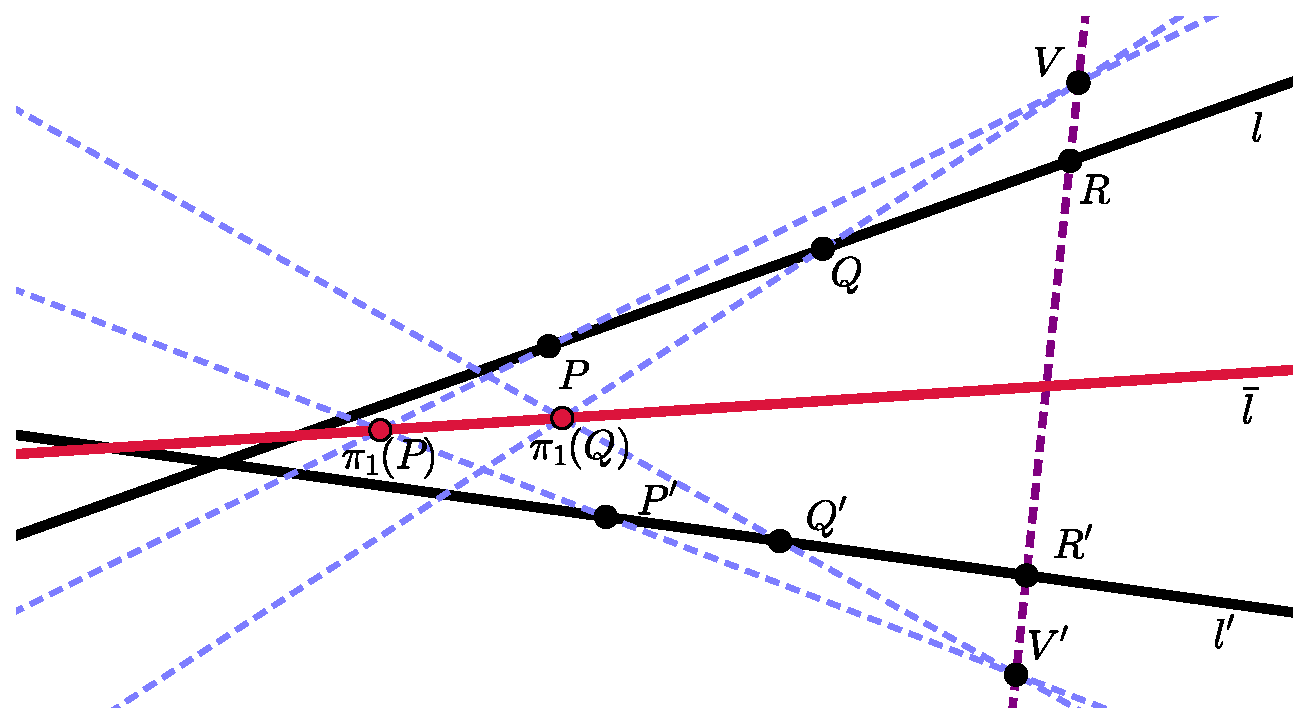
\includegraphics[scale=.4]{Graficos/factorizacion.eps}
	\caption{Ilustración de la prueba de la proposición \ref{C7_prop_factorizacion}.}
	\label{C7_img_factorizacion}
\end{figure}
\begin{obs}[No Unicidad de la Factorización]
	Es importante observar que la factorización de una homografía como composición de perspectividades no es, ni mucho menos, única. Basta tomar otros puntos $V$ y $V'$ como centros de las perspectividades.
\end{obs}
\begin{obs}[Homografías ``Automórficas'']
	\label{C7_obs_automorficas}
	Nótese que la demostración de la proposición \ref{C7_prop_factorizacion} hace uso de que las rectas $l$ y $l'$ son distintas. Esto quiere decir que, por ahora, no podemos decir que una homografía de una recta en sí misma pueda ser factorizada como composición de perspectividades. Dicho pedantemente, no sabemos si el grupo proyectivo o \ti{grupo de homografías} de una recta está generado por perspectividades.
\end{obs}
Vemos a continuación una consecuencia bastante importante (pues resulve el problema planteado en la observación \ref{C7_obs_automorficas}) de la proposición \ref{C7_prop_factorizacion}.
\begin{cor}[Segundo Teorema de Factorización]
	Una homografía $h:l\to l$ (siendo $l$ una recta de $\proy^2$) puede generarse como composición de, a lo sumo, tres perspectividades.
\end{cor}
\begin{proof}
	Consideremos $l'$ cualquier recta distinta de $l$. Tomemos asimismo un punto $V$ que no se encuentre ni en $l$ ni en $l'$. Planteamos la perspectividad $\pi_V$ de centro $V$, que nace en $l$ y muere en $l'$. Para poder trabajar cómodamente caractericémosla por sus imágenes de tres puntos distintos de $l$, a los que llamaremos $P,Q$ y $R$. A dichas imágenes las llamaremos $P',Q'$ y $R'$ respectivamente.
	
	Ahora tomemos la homografía $h':l'\to l$ definida por las condiciones:
	\[\begin{array}{ccc}
	P'\mapsto P\qquad&\qquad
	Q'\mapsto Q\qquad&\qquad
	R'\mapsto R
	\end{array}\]
	Es claro que $h=h'\circ\pi_V$, pero como $h'$ es homografía, basta aplicar la proposición \ref{C7_prop_factorizacion} para obtener que:
	\[h=\pi_1\circ\pi_2\circ\pi_V\]
	Como todas son perspectividades, hemos terminado.
\end{proof}
\section{Teorema del Eje}
\label{C7_Eje}
Para finalizar el capítulo enunciemos y demostremos el llamado ``Teorema del Eje''
\section{Otras Demostraciones del Teorema de Desargues}